\chapter{Vyhodnocení práce}

Výsledkem této práce je implementace systému pro porovnávání výkonu verzí softwaru
pojmenovaná PerfEval. V této kapitole bude krok za krokem ukázáno, jak se systémem pracovat.

\section{Používání systému PerfEval}

V~následujících dvou ukázkách bude vysvětleno, jak používat PerfEval. První ukázka bude
cílit na~nastínění, co~nejjednoduššího použití. Druhá část ukáže aplikaci PerfEvalu na~skutečném projektu.

\subsection*{Jednoduché použití PerfEvalu}

Následující kód popisuje obvyklou posloupnost příkazů práce se systémem PerfEval.
Na začátku je nutné jej inicializovat. PerfEval bude inicializován pro použití JMHJSONParseru.
Následně se přidají výsledky měření několika (alespoň dvou) různých verzí.
Nakonec program vypíše, jestli výkonnostní testy prošly nebo ne.

\begin{lstlisting}
    perfeval init --benchmark-parser JMHJSONParser
    perfeval index-all-results --path tests/old_test --version old_version
    perfeval index-all-results --path tests/new_test --version new_version
    perfeval evaluate && echo "Performance test passed" | exit 0
    echo "Performance test failed" | exit 1
\end{lstlisting}

\subsection*{Návrh skriptu pro doměření výsledků}

Následující kód nastiňuje možnost využití příkazu list-undecided. Výstupem tohoto příkazu
jsou dva tabulátorem oddělené sloupce. V prvním sloupci jsou názvy metod, pro něž systém
eviduje málo naměřených běhů. Ve druhém sloupci je uveden tento počet. Příkaz je určený
pro skriptování, proto není dodaná žádná další hlavička.

V případě, že výstupem není žádný výpis, tak je hodnot u všech testovacích metod naměřeno dostatek. Druhou alternativou
je, že v důsledku nastavení v~konfiguračním souboru systém vyhodnotil, že není možné požadovaný
počet testů doměřit. Následné vyhodnocení pak bude vyžadovat kontrolu uživatelem, protože
systém PerfEval bude vyhodnocení považovat za nevyhovující.

Skript projde všechny řádky výpisu. Pokud je výpis prázdný, tak skončí.
V~následujícím kódu je celá situace velmi zjednodušena. Nalezne se maximální počet
testů, který je zapotřebí změřit. Pro~tento maximální počet se změří výkony obou verzí znovu. Výsledky těchto měření
se zaznamenají do~systému PerfEval. Po~doběhnutí všech měření skript skončí. Vyhodnotí mezi sebou výsledky těchto
verzí a~skončí. Parametry \$1 a~\$2 jsou stará a~nová verze k~porovnání. Předpokládá se, že
příkaz measure provede měření verze zadané jako první argument a~výsledek uloží do souboru specifikovaného jako druhý argument.

\begin{lstlisting}
    #!/bin/bash

    index=1
    while true; do
        output=$(perfeval list-undecided --old-version "$1" --new-version "$2")
        if [[ -n "$output" ]]; then
            max=$(echo "$output" | cut -f2 -d$'\t' | sort -n -k | head 1)
            for ((i=1; i<=$max; i++)); do
                result_file="old_version_$index"
                measure "$1" "$result_file"
                perfeval index-new-result --path "$result_file" --version "$1"

                result_file="new_version_$index"
                measure "$2" "$result_file"
                perfeval index-new-result --path "$result_file" --version "$2"
                ((index++))
            done
        else
            perfeval evaluate --old-version "$1" --new-version "$2"
            exit $?
            break
        fi
    done

\end{lstlisting}

\section{Nasazení systému v praxi}

V~této kapitole bude ukázáno, jak systém PerfEval funguje při~svém nasazení.
Pro ukázku byl vybrán projekt Crate \cite{crateDB}. Jedná se~o~databázový projekt
volně dostupný na platformě GitHub.

Projekt Crate byl vybrán, protože je volně dostupný, a~protože má implementované výkonnostní testy.
Tyto testy je možné spouštět samostatně přímo z~adresáře projektu a~to~i~pro~starší verze.

Systém PerfEval tedy bude použit pro porovnání vybraných commitů. Cílem tohoto
spouštění je zjistit, jestli systém PerfEval detekuje zhoršení a~případně zlepšení
výkonu.

\subsection{Výběr commitů}

Commity pro prezentování práce systému byly vybírány z~období od~21.~dubna 2020 do~11.~května 2023.
Byly vybrány ty commity, jejichž commit message obsahuje slovo „performance“ a~jejich sousední commity (pro porovnání).
Commity byly vybírány z~hlavní větve projektu. Všechny výkonnostní testy byly prováděné na~strojích stejného druhu a~konfigurace.

Z takto vybraných commitů byly dále vybrané jen ty, u~kterých bylo možné projekt bez problémů sestavit. Zároveň bylo také nutné,
aby bylo možné sestavit a~spustit výkonnostní testy. Nakonec tedy bylo vybráno a~naměřeno celkem 16 commitů z~uvedeného období.
Pro každý z~těchto commitů, který reprezentuje v~doméně systému PerfEval verzi, bylo měření provedeno celkem osmkrát.

\subsection{Porovnatelné commity}

Systém PerfEval porovnává pouze dvě verze jejichž všechny testované metody se shodují. Pokud se tedy mezi dvěma
verzemi název některé metody změnil, byla přidaná nová metoda nebo byla nějaká metoda odstraněna, tak tyto verze
PerfEval neporovná.

Proto i ze zvolených 16 commitů nebylo možné porovnat každý s každým. Naměřené commity se tedy rozdělily do tří skupin.
V těchto skupinách se všechny měřené metody shodují, a tak je možné je vzájemně porovnat. Zároveň se v commitu
označeném jako HEAD, tedy nejnovější verze, přidala jedna nová metoda, a tak není možné jej porovnávat s žádným jiným commitem.

V první skupině se nachází 3 commity z období od 8. června 2022 do 4. července 2022.
Ve druhé skupině se nachází 3 commity z období od 28. února 2023 do 7. března 2023.
V poslední skupině se nachází 9 commitů z období od 29. března 2023 do 11. května 2023.
U nejnovějšího commitu z 11. května 2023 (čas 15:42:16) je součástí commit message také poznámka o tom,
že byla přidaná nová testovací metoda v rámci benchmarku JMH.

\medskip

První skupina commitů:
\begin{itemize}
    \item commit 5f0d8a0792f5c6fa2f90f42518b39abb242f21c2 - 8. června 2022
    \item commit 43a996010438ab8784c19269cab14932e02d3a6a - 4. července 2022
    \item commit a9ae6e07bfafea8771f559122f5330a89793748b - 4. července 2022
\end{itemize}

Druhá skupina commitů:
\begin{itemize}
    \item commit f626ec8918422ca0cb6ada5aa7fc601bbbfc53fa - 28. února 2023
    \item commit 03c913ecc91043b1cecdff738dd7bdea07857a9b - 7. března 2023
    \item commit 270b1bd3db98ccd7e2427c7f5a8137d47477b5a1 - 7. března 2023
\end{itemize}

Třetí skupina commitů:
\begin{itemize}
    \item commit 4a4848d9b9c47e4b3e5a00fb4ca0e19e2c11828b - 28. března 2023
    \item commit da83f1eb1d70462d326946a8aa46955e81080f7f - 29. března 2023
    \item commit 5b73ac03409c41acb51b4efd9f58d68c6bffb6b9 - 11. dubna 2023
    \item commit 5b6458b20779a1429fa5724c447bbb9b779298e9 - 4. ledna 2023
    \item commit 50e3ed3a43f7a85d52c6cd96791a4fe76c941ba8 - 12. dubna 2023
    \item commit 6a2b489d9b5691f9bc517e312c86814d4a4f8b07 - 12. dubna 2023
    \item commit df0635dec721861d1f9f5fbde4e9e8647bfebc13 - 10. května 2023
    \item commit 30081686c6e38b3b20817d86a3a38eb652c8625a - 11. května 2023
    \item commit 5ad19461d9bbdfd812586612f3598ef91fb1d529 - 11. května 2023
\end{itemize}

\subsection{Výsledek práce systému PerfEval}

Jednotlivé naměřené hodnoty byly pomocí příkazu \lstinline{index-all-result} přidány do databáze systému PerfEval.
Všechna měření výkonu pro jeden commit byla takto přidána jako výsledek měření jedné verze.
Následně byly pomocí PerfEvalu porovnány sousední porovnatelné commity.

Při porovnávání naměřených datových sad pro první skupinu commitů bylo zjištěno, že výkonnostní testy prošly.
Pokud by tedy tyto verze v rámci průběžné integrace byly měřeny a porovnány systémem PerfEval, tak by byly úspěšně integrovány.
Popis commitu 43a996010438ab8784c19269cab14932e02d3a6a o~významné změně výkonu PerfEval neprokázal.

Porovnáním naměřených datových sad druhé skupiny commitů bylo zjištěno, že výkonnostní testy prošly.
Pokud by tedy tyto verze v rámci průběžné integrace byly měřeny a porovnány systémem PerfEval, tak by také byly úspěšně integrovány.
Při porovnání po sobě jdoucích commitů nebyla zjištěna žádná výrazná změna výkonu a to ani zlepšení.
Při porovnání nejnovějšího a nejstaršího commitu ze skupiny bylo systémem PerfEval zjištěno, že výkon se výkon zlepšil
v~jedné testovací metodě o~více než 5\,\%.
Pokud se v konfiguračním nastavil parametr \lstinline{improvedPerformance} na TRUE, tak program skončil s~nenulovým exit kódem.
PerfEval tedy zjištěné zlepšení nahlásil.

Při porovnávání sousedních verzí ve třetí sadě bylo hlášeno jedno zhoršení výkonu.
Při srovnání commitu 6a2b489d9b5691f9bc517e312c86814d4a4f8b07 a~commitu df0635dec721861d1f9f5fbde4e9e8647bfebc13
bylo systémem PerfEval zjištěno a hlášeno zhoršení výkonu. Ve třech testovacích metodách bylo zjištěno zhoršení výkonu
větší než 5\,\%. Při pohledu na výsledek porovnání je ale také vidět, že se výsledek zlepšil také ve třech testovacích metodách.
Pokud by byl parametr \lstinline{tolerance} nastaven na hodnotu 0,1, tak by ale PerfEval žádnou chybu nehlásil, protože
zhoršení výkonu bylo v~těchto třech testovacích metodách vždy menší než 10\,\%.

Metody u kterých nástroj detekuje zhoršení:
\begin{itemize}
    \item io.crate.execution.TimePrecisionIncreaseTest.currentTimeMillisNextGen
    \item io.crate.data.join.\-RowsBatchIteratorBenchmark.measureConsumeHash\linebreak InnerJoin
    \item io.crate.analyze.PreExecutionBenchmark.measure\_parse\_simple\_select
\end{itemize}

V konečném důsledku tedy nástroj Perfeval odhalil zlepšení výkonu u tří metod o více než 10\.\% a současně zhoršení u výše zmíněných metod, které jsou
součástí výkonnostních testů projektu Crate. Při změně nastavení nástroj byl schopen detekovat i samostatné zlepšení.
Nástroj Crate by tedy bylo možné uplatnit v rámci průběžné integrace projektu.

\begin{figure}
    \centering
    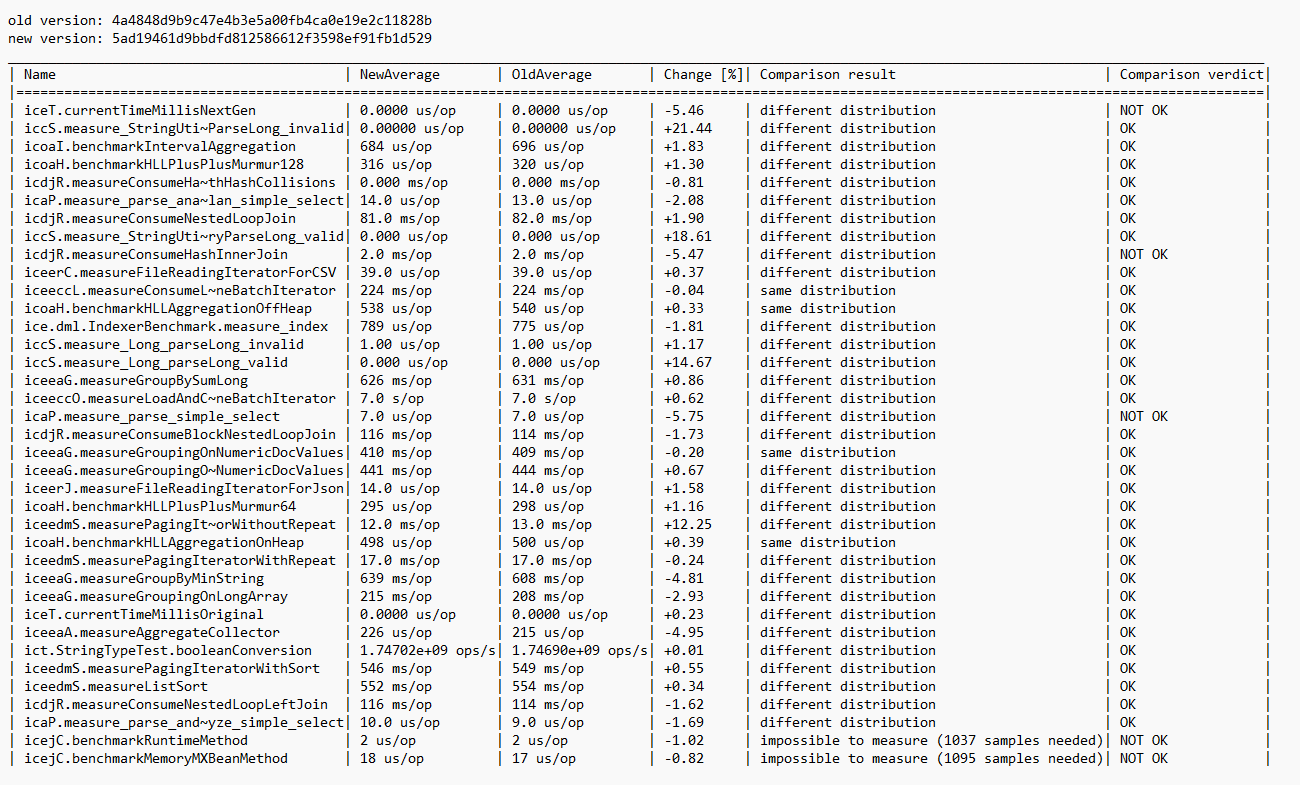
\includegraphics[width=1.5\textwidth, angle=270]{../img/example-table.png}
    \caption{Výsledek porovnání výkonu metod projektu Crate s tolerancí 0,05}
\end{figure}

\begin{figure}
    \centering
    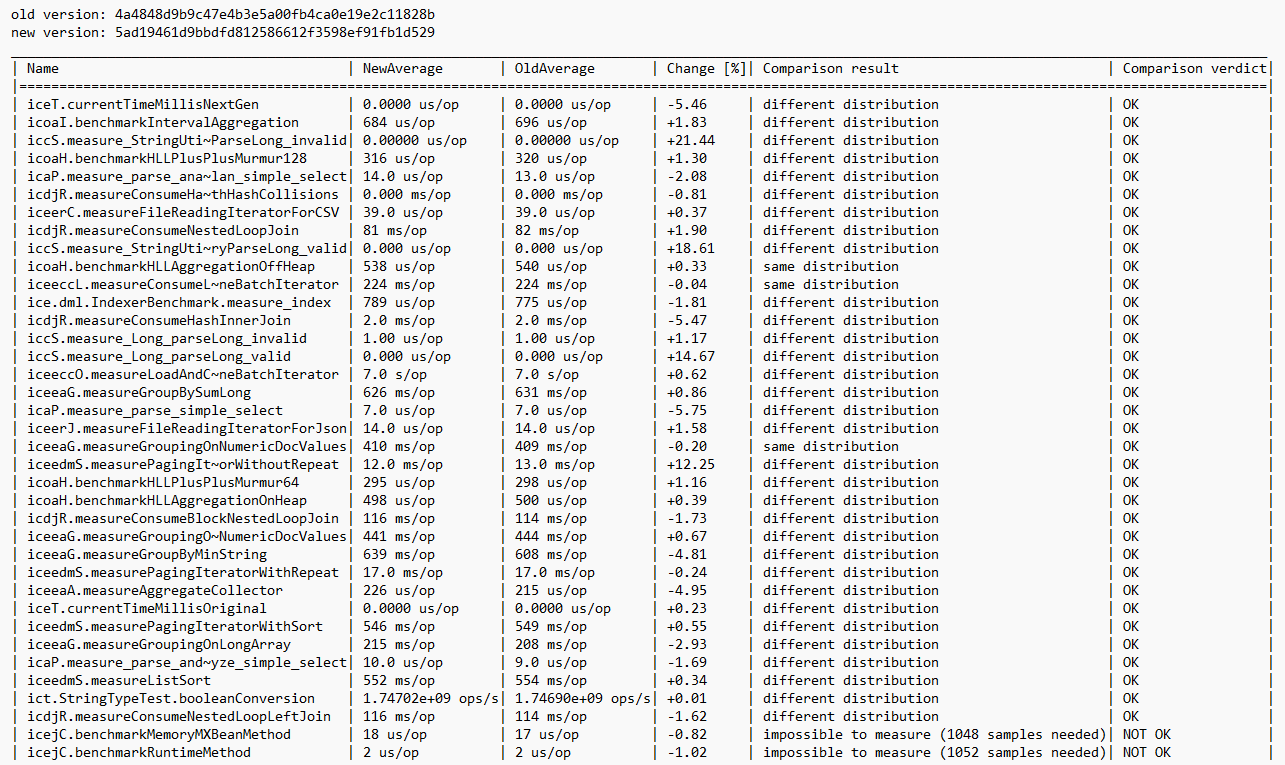
\includegraphics[width=1.5\textwidth, angle=270]{../img/example-table-higher-tolerance.png}
    \caption{Výsledek porovnání výkonu metod projektu Crate s tolerancí 0,1}
\end{figure}